\section{Evaluation}

In this chapter we present an evaluation of our approach. Our evaluation comprises two parts: (i) a usability evaluation involving two experiments with two groups of students (Section~\ref{sec:usab}); and (ii) a preliminary analysis of the performance overhead of our approach (Section~\ref{sec:perf}).  The exact input, instructions, and any additional document we have used in this section are available in appendices or in our repository~\cite{repo}.

\subsection{Usability Evaluation}\label{sec:usab}

We ran empirical evaluation to measure the efficiency of deadlock exceptions with regard to problem solving speed and accuracy. We defined two research questions for this evaluation: 

\begin{itemize}
\item {\bf RQ1.} Is the time spent to identify the bug reduced using our implementation?
\item {\bf RQ2.} Is the accuracy in the identification of the causes of a deadlock bug improved for developers using our approach?
\end{itemize}

The metric we watched to answer the first question was the time (in seconds) to finish each question in the test. For the second question, the metric we used was the number of correct answers. We evaluated students answers under different criteria (see Table~\ref{tab:crit}), where each one received a score that was either 0, 0.5 or 1, where 0 means the criteria was not met at all, 0.5 means it was partially met, and 1 means it was complete. Whenever $(A - B) + C \geq 1.5$ was true, we defined it as a correct answer; that is, whenever the bug was described as deadlock and at least one of the methods involved in the deadlock were identified correctly. We didn't use criteria \emph{D} and \emph{E} because in our questions statements, we didn't make it clear that we wanted description of all locks involved in the deadlock; also, our deadlock implementation at that time only guaranteed at least one thread raising deadlock exception thus affecting at least one method. In other words, this equation means that an answer was correct whenever the bug was described as deadlock, did not contain any affirmation saying it was another type of bug, and at least one of the methods involved were identified.

\begin{table}
\begin{center}
\caption{Criteria to evaluate students answers}\label{tab:crit}
\begin{tabular}{|l|l|}
\hline
Criteria & Description \\
\hline
A & Correctly classified problem as deadlock \\
B & Classified problem as different from deadlock  \\
C & Correctly identified method calls involved in the deadlock \\
D & Correctly identified locks involved in the deadlock  \\
E & Pointed unrelated methods as part of the deadlock \\
\hline
\end{tabular}
\end{center}
\end{table}

\subsubsection{Time Analysis.}

We defined the following hypothesis to answer {\bf RQ1}:

\begin{equation}
  H_{0} : \mu_{TimeLockA} \geq \mu_{TimeLockB}
\end{equation}
\begin{equation}
  H_{1} : \mu_{TimeLockA} < \mu_{TimeLockB}
\end{equation}

\subsubsection{Design, Instrumentation and Subjects.}

In order to prevent \emph{bias}, we needed to control a few factors during the experiment execution. The first factor was the selection of subjects to participate on this experiment, as different background knowledge could potentially influence chosen metrics. The second factor we had to control was the complexity of programs that each subject would have to look into. Complexity was interpreted as a direct relation to the amount of files in the program, number of threads and number of locks to analyze; as we've assumed that easier programs could have little or no benefit from deadlock exceptions, we wanted to have one program that we considered easy to identify the problem and another that was more complex and composed by many files and classes, reflecting a more realistic case. We provided implementations of each program using either \emph{LockA} or \emph{LockB}: the two possible treatments that we wanted to compare.

We decided to use Latin Square Design~\cite{box} to control these two factors mentioned earlier: subjects and program complexity factors. Since we had N subjects, 2 programs and 2 possible treatments, we disposed subjects in rows and programs in columns of latin squares, randomly assigning in each cell of the square a treatment that could be \emph{LockA} or \emph{LockB}, but also guaranteeing that for any given row or column in this square, each treatment appears only once (see Table~\ref{tab:latin}). Consequently, we have replication, local control and randomization which are the three principles of experiment design \cite{box}.

\begin{table}
\begin{center}
\caption{Latin Square design}\label{tab:latin}
\begin{tabular}{|l|l|l|}
\hline
 & Program 1 & Program 2\\
\hline
Subject 1 & LockA & LockB\\
Subject 2 & LockB & LockA\\
\hline
\end{tabular}
\end{center}
\end{table}

We wrote two programs with different complexity which were presented in the same order for all subjects. The first program, known as \emph{Bank}, contained 4 classes spread in 4 files, 3 threads, 3 explicit locks, and 82 lines of code in average. The second program, known as \emph{Eclipse} had 15 classes spread in 11 files, 4 threads, 5 explicit locks, and 40 lines of code in average. We expected the first program to be easier to identify the deadlock because it contained fewer classes and files. Each program could use either \emph{LockA} or \emph{LockB} but we randomly assigned a group to each student so that if they fall into group A, they would start with \emph{LockA} in the first question, but change to \emph{LockB} on the second question; or if they fall in group B, they they would start with \emph{LockB} and switch to \emph{LockA} in the second question. We randomly paired subjects in tuples composed of one subject in group A and another subject of group B, then we created latin squares for each one of these pairs, where any remainders were discarded.

% TODO: insert each program description here, where the deadlock was, etc. in the end, point to where the source for each pdf is %

We repeated this experiment twice.
The two experiments had similar setups but differed in terms of the subjects. For the first experiment, the subjects comprised a group of third-year undergraduate students who underwent an 18-hour concurrent programming course. The course included a number of programming assignments. The experiment was conducted as a test for the course. The subjects of the second experiment were  graduate students enrolled in master's degree or PhD program attending a 40-hour Parallel Programming course with a focus on algorithms and data structures. They had classes about advanced concepts of parallel programming and had practical exercises, including implementing a number of different locking approaches. The participants in the second experiment were all volunteers and were not required to take part in it. Also, for both experiments, the assignments were the same. It asked students to identify any problems they could with the provided programs.

%We did a survey with the second group to understand their background even further (see charts below) at the end of the experiment. TODO: insert chart with survey results

\subsubsection{Metrics Collection.}

All students started the experiment with program \emph{Bank}. When they finished, they received the second program, \emph{Eclipse}. When a student finished one of the programs, we set a timestamp on it, or in a few cases, we allowed students to do it by themselves but we had to double check the values and fix in case there was any error. The timestamp was written based on a chronometer visible to everyone in the laboratory. For the first group (undergraduate students), we allowed 90 minutes per program. For the second group (graduate students), we allowed 60 minutes per program. 

Each one should start the experiment with the first question containing \emph{Program 1} and once they finish to provide an answer, they should request for the second question. At that point, we collect and place a timestamp in their answer. Once they finish the second question containing \emph{Program 2}, then they should again give us a notice so we can leave a new timestamp. Later we used these timestamps to measure how long they took to finish each question. We have started this experiment with a time limit for each question of 60 minutes each. However, during the first experiment, students complained and we realized it would not be sufficient for all students so we expanded to 90 minutes.

The timestamp was written by students conducting the experiment based on a counter we projected on the laboratory wall in real time. In a few circunstances the subject could write the timestamp when they finished, but we have double checked the value at the time we collected their answer, overwriting in case they did any mistake.

\subsubsection{Experiment Operation.}

We executed this experiment in two different days. In the first day we did it with undergraduate students in replacement of their default exam, so their participation was obligatory but we disclaimed they could optionally leave a comment if they did not want to take part in this research, so we would not use their data. Fortunately no one chose to not participate. In the second day, we did it with graduate students after the last class of Parallel Programming course and it was optional. In total, 31 students participated on the first day and 16 students participated on the second day, but we had to discard 2 students data because they arrived late and they had to leave early.

On the first day we started with a time frame of 2 hours for the whole experiment, so we decided to set a deadline for each question and put a time limit of 1 hour each. Later we expanded the time limit to 1 hour 30 minutes for each question. On the second day we decided to stick with 1 hour each because there was no demand to extend it.

\subsubsection{Results.}

Time analysis was conducted with R Statistical Software using the inputs extracted from each day.
We used the linear model described in Figure~\ref{fig:model} that considers the effect of different factors
on the response variable as proposed by other authors~\cite{paola}~\cite{sanchez}.

\begin{figure}
\begin{center}
$Y_{lijk} = \mu + \tau_{l} + \tau\alpha_{li} + \beta_{j} + \gamma_{k} + \tau\gamma_{lk} + \epsilon_{lijk}$\\
\vspace{4mm}
\begin{tabular}{ll}
$Y_{lijk}$ & - response of $l_{th}$ replica, $i_{th}$ student, $j_{th}$ program, $k_{th}$ lock \\
$\tau_{l}$ & - effect of $l_{th}$ replica \\
$\tau\alpha_{li}$ & - effect of interaction between $l_{th}$ replica and $i_{th}$ student \\
$\beta_{j}$ & - effect of $j_{th}$ program \\
$\gamma_{k}$ & - effect of $k_{th}$ lock \\
$\tau\gamma_{lk}$ & - effect of interaction between $l_{th}$ replica and $k_{th}$ lock \\
$\epsilon_{lijk}$ & - random error \\
\end{tabular}
\caption{Regression model.}\label{fig:model}
\end{center}
\end{figure}

Initially, we've plotted box-plot graphic (Figure~\ref{fig:boxplot1}) and calculated the average time spent to solve tasks for both groups (Table~\ref{tab:mean1}).
They show that students using {\tt LockB} took more time to complete the tasks.
On Figure~\ref{fig:boxplot1}, we can see time spent for both groups stop at nearly the same point, and we believe the reason behind it is that we enforced a time limit for each question.
If there was no such time limit on each question, we believe that {\tt LockB} time spent range would be significantly wider.

\begin{figure}
\centering
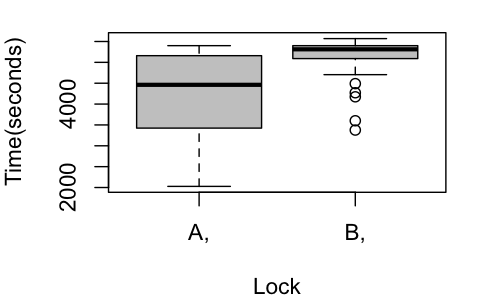
\includegraphics[height=4.5cm]{img/u1.png}
\caption{First experiment box-plot graphic.}\label{fig:boxplot1}
\end{figure}

\begin{table}
\centering
\begin{tabular}{|l|l|l|}
\hline
 & Time Spent (seconds)\\
\hline
LockA & 4227.800 \\
LockB & 5086.367 \\
\hline
\end{tabular}
\caption{First experiment's average time spent}\label{tab:mean1}
\end{table}

Then we run the Box-Cox transformation - a power transformation - to reduce anomalies such as non-additivity and non-normality.
First we verify if the transformation is needed, obtaining the curve in the left of Figure~\ref{fig:transf1}.
Since the value of {\tt lambda} at the maximum point in the curve is not approximately 1, we should apply it.
In order to apply the transformation, $Y_{lijk}$ should be powered to that $\lambda$ on our regression model.
Now, using the transformed model, we obtain the curve shown in the right of Figure~\ref{fig:transf1}.

\begin{figure}
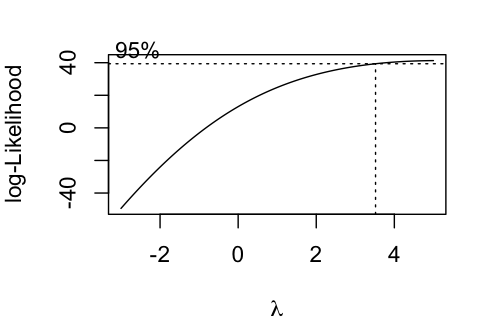
\includegraphics[height=4.5cm, width=6cm]{img/u2.png}
\hfill
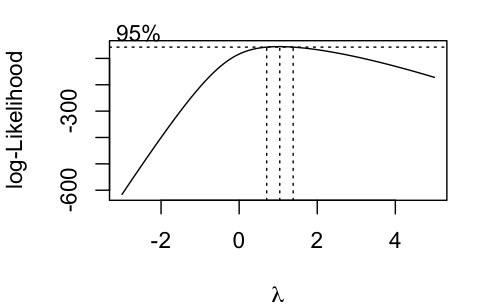
\includegraphics[height=4.3cm, width=6cm]{img/u2boxcox.png}
\caption{First experiment: before and after box-cox transformation ($\lambda = 5$).}\label{fig:transf1}
\end{figure}

In the next step we ran Tukey Test of Additivity to check whether effect model was additive.
Interaction between factors displayed on rows and columns of each latin square won't affect significantly the response only when the model is additive~\cite{box},
so we must verify it (Figure~\ref{tab:tukey}).

\begin{figure}
\centering
\begin{tabular}{ll}
$H_{0}$ & : The model is additive \\
$H_{1}$ & : $H_{0}$ is $false$ \\
\end{tabular}
\caption{Tukey Test of Additivity hypothesis}\label{tab:tukey}
\end{figure}

When the test was executed, we obtained p-value of 0.514, which means we cannot reject $H_{0}$.
Consequently the model was considered to be additive.

Finally, we ran the ANOVA (ANalysis Of VAriance) test which compares the effect of treatments on the response variable,
providing an approximated p-value for every associated factor (see Table~\ref{tab:anova1}).
When a variable has p-value $< 0.05$, it means that factor was statistically significant to the response.
It shows that {\bf lock factor was the most significant to the response}, allowing us to reject our null hypothesis defined in Equation 10.

\begin{table}
\begin{center}
\caption{Undergraduate students experiment ANOVA results.}\label{tab:anova1}
\begin{tabular}{|l|l|l|l|l|ll|}
\hline
                & Df &    Sum Sq  &  Mean Sq   & F value & \emph{p-value} &     \\  
Replica         & 14 & 3.8633e+37 & 2.7595e+36 & 1.6553  & 0.1784197 &     \\   
Program         & 1  & 4.1460e+36 & 4.1460e+36 & 2.4869  & 0.1371197 &     \\   
Lock            & 1  & 3.9489e+37 & 3.9489e+37 & 23.6873 & 0.0002492 & *** \\
Replica:Student & 15 & 4.1013e+37 & 2.7342e+36 & 1.6401  & 0.1808595 &     \\  
Replica:Lock    & 14 & 2.4033e+37 & 1.7166e+36 & 1.0297  & 0.4785520 &     \\  
Residuals       & 14 & 2.3340e+37 & 1.6671e+36 &         &           &     \\
\hline
\end{tabular}
\end{center}
\end{table}

Now we will show the results collected by the second experiment with graduate students. They were exposed to the same set of problems in a different day, but as explained before, they only had a time limit of 1 hour per question.

When we analyze the box-plot for the second group (Image~\ref{fig:boxplot2}) and their average time spent (Table~\ref{tab:mean2}), we can see there was a clear improvement on the time for students using \emph{LockA}.

\begin{figure}
\centering
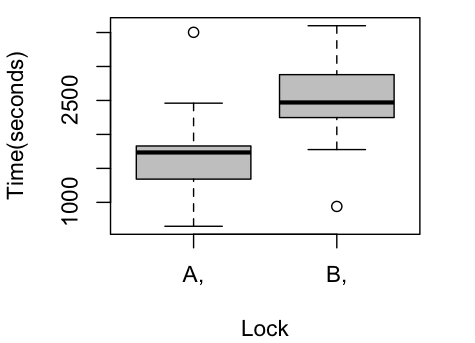
\includegraphics[height=4.5cm]{img/g1.png}
\caption{Second experiment box-plot graphic.}\label{fig:boxplot2}
\end{figure}

\begin{table}
\centering
\begin{tabular}{|l|l|l|}
\hline
 & Time Spent (seconds)\\
\hline
LockA & 1737.714 \\
LockB & 2507.714 \\
\hline
\end{tabular}
\caption{Second experiment's average time spent}\label{tab:mean2}
\end{table}

Moving foward with the analysis, we check if a box-cox transformation is needed. Since the value is not approximately 1, we apply the power transformation the same way we did with the first experiment, but with the corresponding lambda value.

\begin{figure}
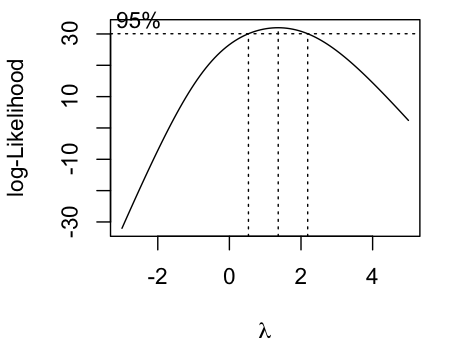
\includegraphics[height=4.5cm]{img/g2.png}
\hfill
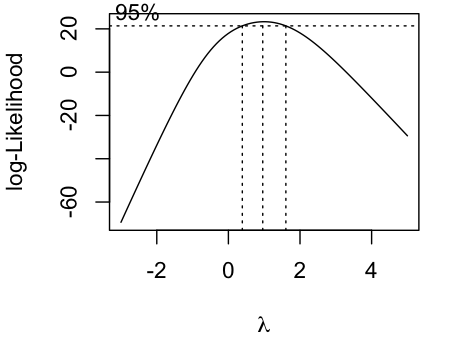
\includegraphics[height=4.4cm]{img/g2boxcox.png}
\caption{Before and after box-cox transformation ($\lambda = 1.3636$).}\label{fig:transf2}
\end{figure}

Finally, running ANOVA, we can see that the type of lock was the most significant factor for the response time, as shown in Table~\ref{tab:anova2}. Again, we can reject the null hypothesis.

\begin{table}
\begin{center}
\caption{Graduate students ANOVA results.}\label{tab:anova2}
\begin{tabular}{|l|l|l|l|l|ll|}
\hline
                 & Df &    Sum Sq &   Mean Sq  & F value &   Pr(>F) & \\   
\hline
replica          & 6 & 2576883250 &  429480542 & 14.1891 & 0.0025793 & **  \\
program          & 1 &    6875586 &    6875586 &  0.2272 & 0.6505035 &     \\
lock             & 1 & 1958179433 & 1958179433 & 64.6938 & 0.0001975 & *** \\
replica:student  & 7 & 2328154077 &  332593440 & 10.9881 & 0.0047601 & **  \\
replica:lock     & 6 &  823830276 &  137305046 &  4.5362 & 0.0441188 & *   \\
Residuals        & 6 &  181610625 &   30268438 &         &           &     \\
\hline
\end{tabular}
\end{center}
\end{table}

\subsubsection{Accuracy Analysis.}

We used the number of correct answers using each lock to measure accuracy, so we defined the following hypothesis to answer {\bf RQ2}. 

\begin{equation}
  H_{0} : \mu_{CorrectAnswersLockA} \leq \mu_{CorrectAnswersLockB}
\end{equation}
\begin{equation}
  H_{1} : \mu_{CorrectAnswersLockA} > \mu_{CorrectAnswersLockB}
\end{equation}

Once we collected all answers, we manually evaluated each one of them according to the criterias established previously, where each criteria had an associated value between 0 and 1. Then we've ran a script that evaluates the equation we defined before to classify whether an answer was correct or not. Grouping the results in tables, we have Table~\ref{tab:acc1} and Table~\ref{tab:acc2}.

\begin{table}
\begin{center}
\caption{Undergraduate students answers accuracy}\label{tab:acc1}
\begin{tabular}{|l|l|l|}
\hline
 & Correct & Incorrect\\
\hline
LockA & 29 & 2\\
LockB & 16 & 15\\
\hline
\end{tabular}
\end{center}
\end{table}

\begin{table}
\begin{center}
\caption{Graduate students answers accuracy}\label{tab:acc2}
\begin{tabular}{|l|l|l|}
\hline
 & Correct & Incorrect\\
\hline
LockA & 13 & 1\\
LockB & 10 & 4\\
\hline
\end{tabular}
\end{center}
\end{table}

Applying Fisher's exact test we can see that undergraduate students results presented a two-tailed P value equals 0.0004: the association between rows (groups) and columns (outcomes) is considered to be extremely statistically significant; consequently, there is clear evidence of improvement on accuracy (see Table~\ref{tab:acc1}).

Meanwhile graduate students results presented a two-tailed P value equals 0.3259, which does not represent a statistically significant evidence of improvement in accuracy (see Table~\ref{tab:acc2}).

% TODO: add script and the data used (anonymized) to appendices or put on github and link %

\subsection{Discussion}

% TODO: review this section, it was written based on older results %

We can see in our results that both groups of students have improved their time to solve the problem when they had the lock with deadlock exception. Also, on the first group, we have found statistically significant evidence that it improved answers accuracy, but not for the second group.

We cannot draw conclusions regarding the improved accuracy on the second group, but we can bring up some relevant aspects we've observed and make a few hypothesis. Some students in the second group were greatly experienced on concurrent programming and they knew how to efficiently find a deadlock using the tools available in Eclipse. Thus, they have finished the exercise really quickly for both problems, knowing exactly which points in the code were involved in the deadlock. So we can see that deadlock exceptions are more helpful for unexperienced programmers in general, and it's possible that even if we had a bigger sample for the second group, we would still not see a significant difference that would indicate deadlock exceptions improved their accuracy.

However, we believe that the benefits of deadlock exceptions are beyond helping unexperienced programmers to find deadlocks more precisely. Experienced programmers would still benefit in many cases where the deadlock is not as obvious as in the exercise we've presented. For example, in a more realistic situation, a deadlock can happen in a background thread that doesn't really affect the program execution overall but make the execution lacking some expected behavior. Furthermore, in non-interactive systems where they are only running in background, is nearly impossible to know when there's a problem unless this software is monitored constantly which is very time consuming or the system produces output constantly that is affected by a potential deadlock. If we have a deadlock exception, we can either prepare and handle this exception on the code level, or just have this signal from output that would help developers to fix it later.

\subsection{Threats To Internal Validity}

In this experiment, we've collected evidence on how the presence of deadlock exception affects student ability to identify deadlocks accurately. However, we must raise a few considerations regarding the validity of our results.

\subsubsection{Time Measurement.}

Since we wanted to run the experiment in a homogenous environment, we've decided to run it in a laboratory in Federal University of Pernambuco, and we've provided links to download the exercise and a few instructions explaining how to deploy it. We wanted to make it as easy as possible and before we've started the test, we gave a small presentation reproducing step by step the instructions that would be described on each exercise, so everyone could follow up and make the setup at the same time. Once everyone was done, we've started to count the time and allowed them to run the programs and start debugging. However, this procedure was not enough: there was a few students (approximately 3 in total) who did the setup differently and could not execute the program; therefore, they've lost a few minutes until we've fixed that for them. Since they've lost only a few minutes, we have still counted them as part of the experiment and did not discount the time.

Furthermore, some students arrived at the test more than 10 minutes late. We've allowed them to join, but some of the remaining computers in the laboratory had issues like they were not logging in or the mouse was not working. We've lost a few minutes to make them work or find a new computer and once each of them did the setup, we've started to count their time individually.

Whenever a student finished a given question, if the time was below the time limit they had available, we have marked the current timestamp on each student's name in the whiteboard. Each entry inserted was already sorted by time, so we easily tracked whether each student was close to the second question's time limit. It would have been better to do this automatically rather than doing manually, so we could potentially reduce overhead of these timestamp operations and increase their precision.

Also, we believe that our imposed time limit have limited more drastically the time ranges on the first group because they spent more time on each question. Also the fact it was an exam for them may have delayed the time to answer because they were more careful. We have observed during the experiment that many students wrote their answers but they were reluctant to ask for the next question because they still have plenty of time left and they wanted to make sure it was correct. We did not observe such behavior with the second group of students and we believe it is because they did not have the same pressure to deliver correct results as the first group had.

\subsubsection{Exercises.}

We understand that the two questions we've used to evaluate the students are far easier than what most software engineers have to deal with in the real world. However we could not use any real world issue because it would easily take the time limit of the experiement for each bug.

On the other hand, we've created two questions based on real world bugs that we have found while searching for deadlock bugs in open source repositories. Each question had a particular level of granularity, where one should be easier to find a bug because of the less amount of code to examine and another that should be more difficult because of the reasonable amount of different files to look at.

Some researchers actually believe that empiric evaluations should not be limited to real projects. Buse claims there are benefits of using non-real artifacts \cite{buse} because it's easier for researchers to translate research questions into successful experiments as it allows a greater control over confouding factors. Otherwise, it would be necessary to turn all participants familiar with the codebase of a real and complex system before even starting the experiment. 

\subsection{Threats to External Validity}

Let's consider a few conditions that might limit the generalization power of our findings in this experiment.

\subsubsection{Students.}

Each student which participated in this experiment had a different background. What we did to minimize the differences was to select groups where students had at least basic experience in concurrent programming and they should be familiarized with the types of bugs such codes can have: the first group of students with undergraduate students attended the class Paradigms of Computaional Languages where deadlocks are covered in classes and exercises; the second group with graduate students attended the class Parallel Programming which covered concurrent programming in low level detail in classes and exercises, including deadlock detection.

Some studies have already addressed the problem of drawing conclusions made with students but some suggest that using students as subjects is as good as using industry professionals \cite{staron}. Runes ran an experiment which shows that there's not much significant differences between undergraduate, graduate and industry professionals, with the exception that undergraduate students often take more time to complete the tasks \cite{runes}.

\subsection{Performance Overhead}\label{sec:perf}

We conducted a preliminary set of experiments to analyze the overhead of our approach.
We compared the our implementation of ReentrantLock with deadlock exceptions, the original ReentrantLock and Eclipse's {\tt OrderedLock}~\cite{orderedlock} implementation in a synthetic benchmark.

OrderedLock is a deadlock-safe implementation of a lock which relies on Eclipse's code architecture.
It is similar our approach in the sense that it attempts to detect deadlocks at runtime. However, it aims to be general, detecting $N$-thread deadlocks without much concern for performance: when a deadlock happens, it releases all locks by a given thread and suspends it, allowing other threads to proceed;
later, the suspended thread will acquire such locks again.
Since it allows threads to temporarily give up all its owned locks, it loses the property of guaranteeing exclusive access policy in \emph{critical zones} that all locks should provide.
In order to use it in our evaluation, as it deeply relies on Eclipse's code architecture to function, we had to perform some small code changes, removing only Eclipse-specific bits that did not affect the core functionality of OrderedLock.
The source code for these lock implementations is available elsewhere~\cite{repo}.

We developed a synthetic benchmark that creates \emph{N} threads that perform additions to ten integer counters where each increment in a counter is protected by explicit locks. Each thread would have to increment its corresponding counter 1000 times before finishing its execution and the counters were evenly distributed across the threads. Therefore, each counter will have exactly \emph{(N / 10)} threads doing increments on it and higher values of \emph{N} result in higher contention, that is, more threads will compete against each other for a particular counter. In this preliminary evaluation, we have conducted measurements for values of $N$ equal to 10, 50, 100, and 200. Since each thread in the benchmark never acquires more than one lock at the same time, deadlocks cannot occur. We emphasize that this setup is very conservative, since every operation that each thread performs requires locking. Thus, the obtained overhead will be a worst-case estimate and thus much higher than one would encounter in a real-world application~\cite{lozi}. The measurements were made on an Intel CoreTM i7 3632QM Processor (6Mb Cache, 2.2GHz) running Ubuntu 12.04.4 LTS and each cell in Table~\ref{tab:overhead} is the average of 50 executions (preceded by 20 executions that served as a warm-up).

\begin{table}
\begin{center}
\caption{Benchmark time measurements (in seconds)}\label{tab:overhead}
\begin{tabular}{|l|l|l|l|}
\hline
\# Threads & ReentrantLock & ReentrantLock Modified & OrderedLock \\
\hline
10 & 0.084184 & 0.105729 & 0.159503\\
50 & 0.089094 & 0.136507 & 1.094718\\
100 & 0.090978 & 0.159541 & 3.395974\\
200 & 0.131739 & 0.194075 & 11.258714\\
\hline
\end{tabular}
\end{center}
\end{table}

The difference of results between our implementation and the original ReentrantLock gives a range of increased time from about 50\% to 90\%. Meanwhile, OrderedLock performed a lot worse, reaching a 8446.3\% increase in time for the worst case. To get a rough estimate of the impact that this overhead would have on actual application execution time, we analyzed the results obtained by Lozi et al.~\cite{lozi}. The authors profiled 19 real-world applications and small benchmarks in order to measure the time these systems spend on their critical sections. Worst-case results ranged between 0.3\% and 92.7\%. If we consider the average time spent on the critical sections of 12 of these systems, the impact of our approach on the overall execution time would be \textbf{less than 6\% in the worst case}. The remaining cases are extreme, in the sense that these systems spend more time in their critical sections than out of them~\cite{lozi}. 



